\documentclass{article}
\usepackage{natbib}
\usepackage{graphicx}
\usepackage{tabularx}
\usepackage{changepage}
\usepackage{pdflscape}


\begin{document}
\title{VALET: \emph{de novo} pipeline for finding metagenomic mis-assemblies}
\author{Supplemental Material}
\date{}
\maketitle
\section{VALET Pipeline}
%%%%
%%%% TODO add brief description of pipeline
%%%%

\begin{figure}[tb!]
\begin{center}
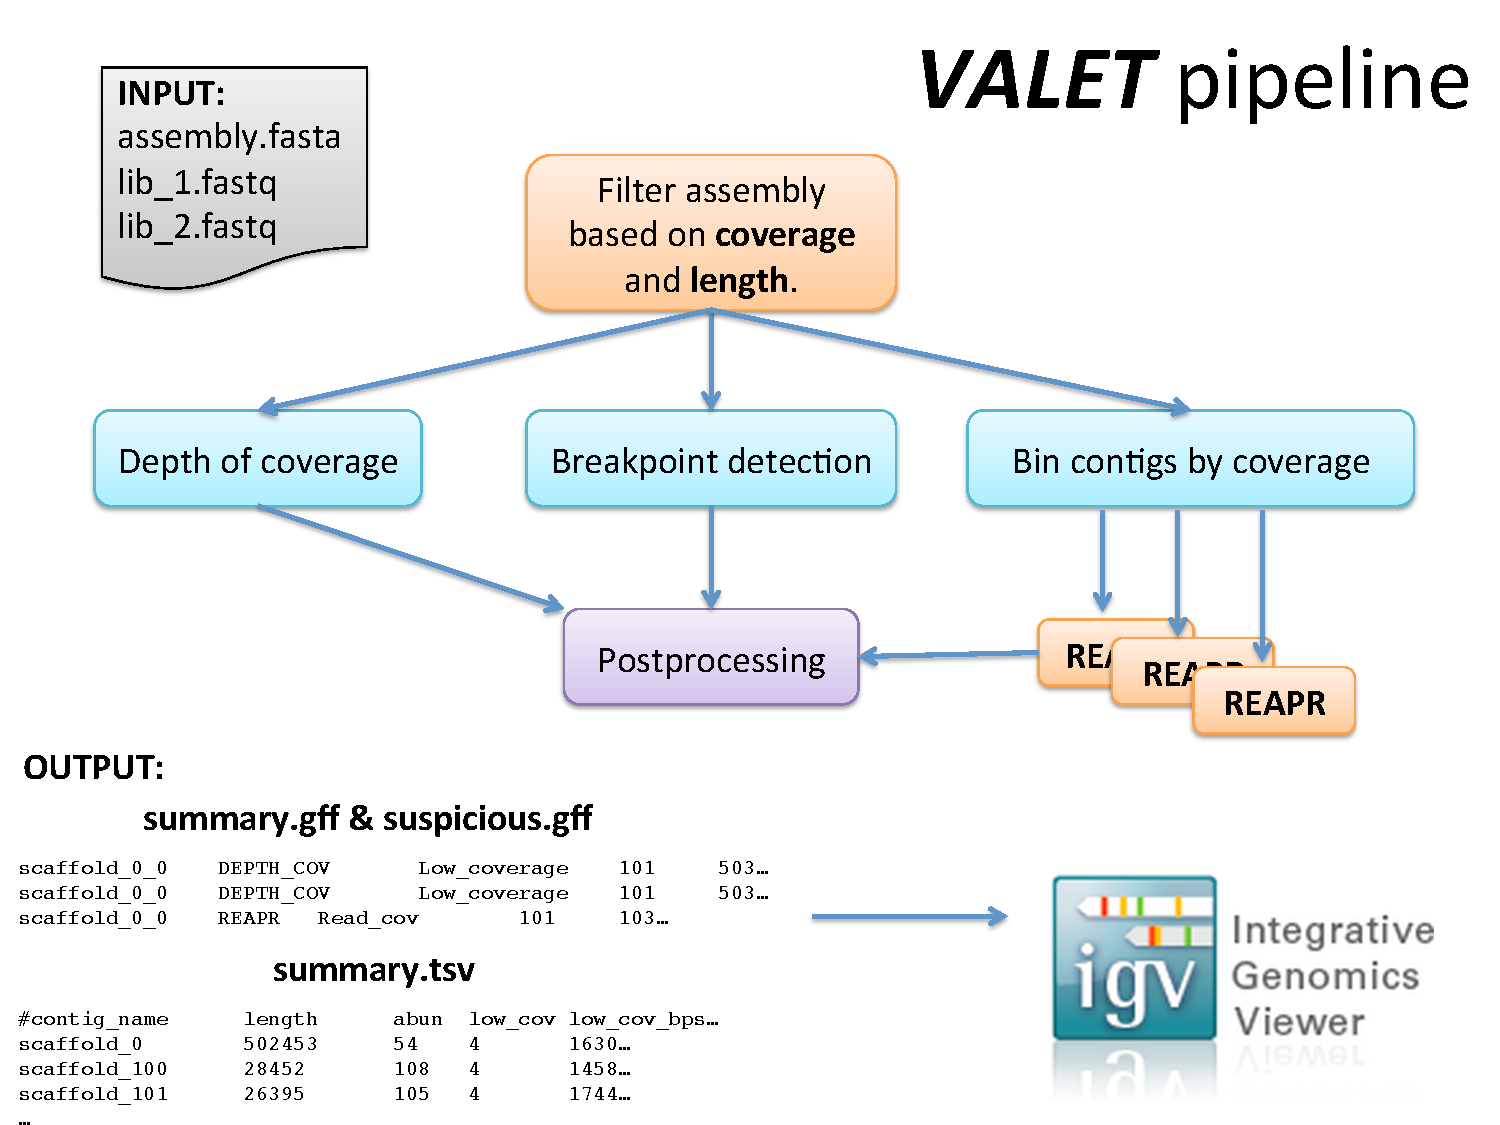
\includegraphics[width=3in]{figures/valet_pipeline}
\end{center}
\caption[valet_pipeline]{Digram of the VALET pipeline.}
\label{fig:valet_pipeline}
\end{figure}

\section{Evaluation}
\subsection{Definition of a mis-assembly}
We compared misassemblies identified by VALET on a simulated and synthetic metagenomic dataset to the reference based metagenome assembly evaluation tool MetaQUAST~citep{mikheenko2015metaquast}.
We ran VALET on the assemblies and compared the errors found with the reference-based mis-assemblies detected by MetaQUAST.
MetaQUAST uses the Plantagora’s definition of a mis-assembly,
i.e., a mis-assembly breakpoint is defined as a position in the assembled contigs where (1) the left flanking
sequence aligns over 1kb away from right flanking sequence on the reference, or (2) the sequences overlap by
over 1kb, or (3) the right flanking sequence aligns on opposite strands or different chromosomes. 
As mutations in the strain in a metagenome can contain structural variants relative to the reference genome. 
MetaQUAST uses the read mapping structural variant caller MANTA~\citep{chen2015manta} to filter canidate misassemblies. 
If any part of a region flagged by VALET overlaps with a mis-assembled region reported by MetaQUAST, we consider it a true positive (mis-assembly correctly identified by our method).
%In addition, the N50 of each assembly is recalculated after breaking at mis-assemblies found by QUAST.

\subsection{VALET achieves high sensitivity on a simulated metagenomic community}
%Evaluating correctness – mock even/staggered/mixture of known communities.
%Examining error composition of all HMP data sets.
%Grab a handful to compare with new assemblies.
%Show that window length doesn’t matter when comparing.
%Does window length matter when comparing assemblies.

We examine the sensitivity of VALET on a toy mock metagenomic community consisting of four bacteria at varying abundances: 80X \emph{Bacteroides vulgatus}  ATCC8482 (Accn. NC_009614.1), 60X \emph{Bacillus cereus} (Accn. NC_003909.8), 40X \emph{Actinomyces odontolyticus} (Accn. NZ_DS264586.1), and 20X \emph{Acinetobacter baumannii} (Accn. NC_009085.1).
Approximately four million reads are simulated using \textsc{wgsim}~\citep{li2013wgsim} with default parameters and 100 bp forward and reverse reads.
The dataset was assembled using Velvet~\citep{zerbino2008velvet}, MetaVelvet~\citep{namiki2012metavelvet}, MaSuRCA~\citep{zimin2013masurca}, and SOAPdenovo2~\citep{luo2012soapdenovo2} by MetAMOS~\citep{treangen2013metamos}.

%%%%%%%%%%%%%%%%%%%%%%%%%%%
%% TODO Assembly values
%%%%%%%%%%%%%%%%%%%%%%%%%%%
Across all assemblers, VALET detects greater than 80\% of mis-assemblies detected by MetaQUAST (Table~\ref{simulated_community}).% with all mis-assemblies being found in the IDBA-UD and SOAPdenovo2 assemblies.
%IDBA-UD, MetaVelvet, and SPAdes assemblies contain roughly the same amount of sequence (16.3-16.5 Mbp), while SOAPdenovo2 contains roughly 4 Mbp less.
IDBA-UD has the greatest N50 after breaking the assembly at regions marked by QUAST (206.7 Kbp), followed by SPAdes (128.1 Kbp), MetaVelvet (29.5 Kbp), and SOAPdenovo2 (10.8 Kbp).
%IDBA-UD has the greatest NA50 (208.8 Kbp), followed by SPAdes (130.9 Kbp), MetaVelvet (29.5 Kbp), and SOAPdenovo2 (10.8 Kbp)

%%%%%%%%%%%%%%%%%%%%%%%%%%%
%% TODO add figure to repo
%%%%%%%%%%%%%%%%%%%%%%%%%%%
These rankings match those provided by VALET (Figure~\ref{fig:simulated_frc}).

%%%%%%%%%%%%%%%%%%%%%%%%%%%
%% TODO Update table values
%%%%%%%%%%%%%%%%%%%%%%%%%%%

\begin{landscape}
\begin{table}
\centering
\footnotesize
\begin{tabular}{|l|c|c|c|c|c|c|c|c|c|c|c|c|}
  \hline
  \multicolumn{6}{|c}{} & \multicolumn{3}{|c|}{Mis-assembly signatures} & \multicolumn{3}{c|}{Suspicious regions}   &  \\
  \hline
  Assembler   & Len (Mbp) & Ctgs  & N50 (Kbp) & NA50  & Errs & Num   & Valid & Sens     & Num & Valid & Sens    & Mismatches per Kbp \\
  \hline
  IDBA-UD     & 16.5      & 200   & 208.8     & 206.7 & 36   & 804   & 36    & 100.00\% & 25  & 8     & 22.20\% & 23.95              \\
  MetaVelvet  & 16.3      & 1,117 & 29.5      & 29.5  & 21   & 2,802 & 19    & 90.50\%  & 4   & 2     & 9.50\%  & 35.52              \\
  SPAdes      & 16.4      & 330   & 130.9     & 128.1 & 37   & 1,117 & 31    & 83.80\%  & 17  & 4     & 10.80\% & 22.43              \\
  Soapdenovo2 & 12.3      & 2,161 & 10.8      & 10.8  & 1    & 4,983 & 1     & 100.00\% & 2   & 0     & 0\%     & 13.37 \\
  \hline
\end{tabular}
\caption[VALET results for simulated mock community]{VALET results for simulated mock community consisting of four bacteria at varying abundances: \emph{Bacteroides vulgatus} (80x), \emph{Bacillus cereus} (60x), \emph{Actinomyces odontolyticus} (40x), and \emph{Acinetobacter baumannii} (20x). Reads were assembled using the four provided assemblers. General assembly statistics include length in Mbp (Len), number of contigs (Ctgs), N50 contig size (N50), N50 of contigs after broken at mis-assemblies (NA50), number of errors detected by MetaQUAST (Errs), number of flagged regions by VALET (Num), number of flagged regions that overlap an error found by MetaQUAST (Valid), sensitivity (Sens), and mismatches per Kbp.}
\label{simulated_community}
\end{table}

\begin{table*}[tb!]
\centering
\footnotesize
\label{synthetic_valet}
\begin{tabular}{|l|c|c|c|c|c|c|c|c|c|c|c|c|}
  \hline
  \multicolumn{6}{|c}{} & \multicolumn{3}{|c|}{Mis-assembly signatures} & \multicolumn{3}{c|}{Suspicious regions}   &  \\
  \hline
  Assembler & Len (Mbp) & Ctgs   & N50 (Kbp) & NA50 (Kbp) & Errs   & Num       & Valid  & Sens    & Num    & Valid  & Sens    & Mismatches per Kbp \\
  \hline
  MEGAHIT   & 192.3     & 19,145 & 38.9      & 33.5       & 770    & 30,377    & 268    & 34.80\% & 2,239  & 100    & 13.00\% & 92.24              \\
  Omega     & 194       & 10,284 & 44.1      & 11.9       & 56,917 & 1,425,127 & 55,108 & 96.10\% & 17,758 & 13,935 & 96.80\% & 98.55 \\
  \hline
\end{tabular}
\caption[VALET results for assemblies of the Shakya et al.~\citep{shakya2013comparative} dataset]{VALET results for assemblies of the Shakya et al.~\citep{shakya2013comparative} dataset. General assembly statistics include length in Mbp (Len), number of contigs (Ctgs), N50 contig size (N50), N50 of contigs after broken at mis-assemblies (NA50), number of errors detected by MetaQUAST (Errs), number of flagged regions by VALET (Num), number of flagged regions that overlap an error found by MetaQUAST (Valid), sensitivity (Sens), and mismatches per Kbp.}
\end{table*}

\end{landscape}

\begin{figure}[tb!]
\begin{center}
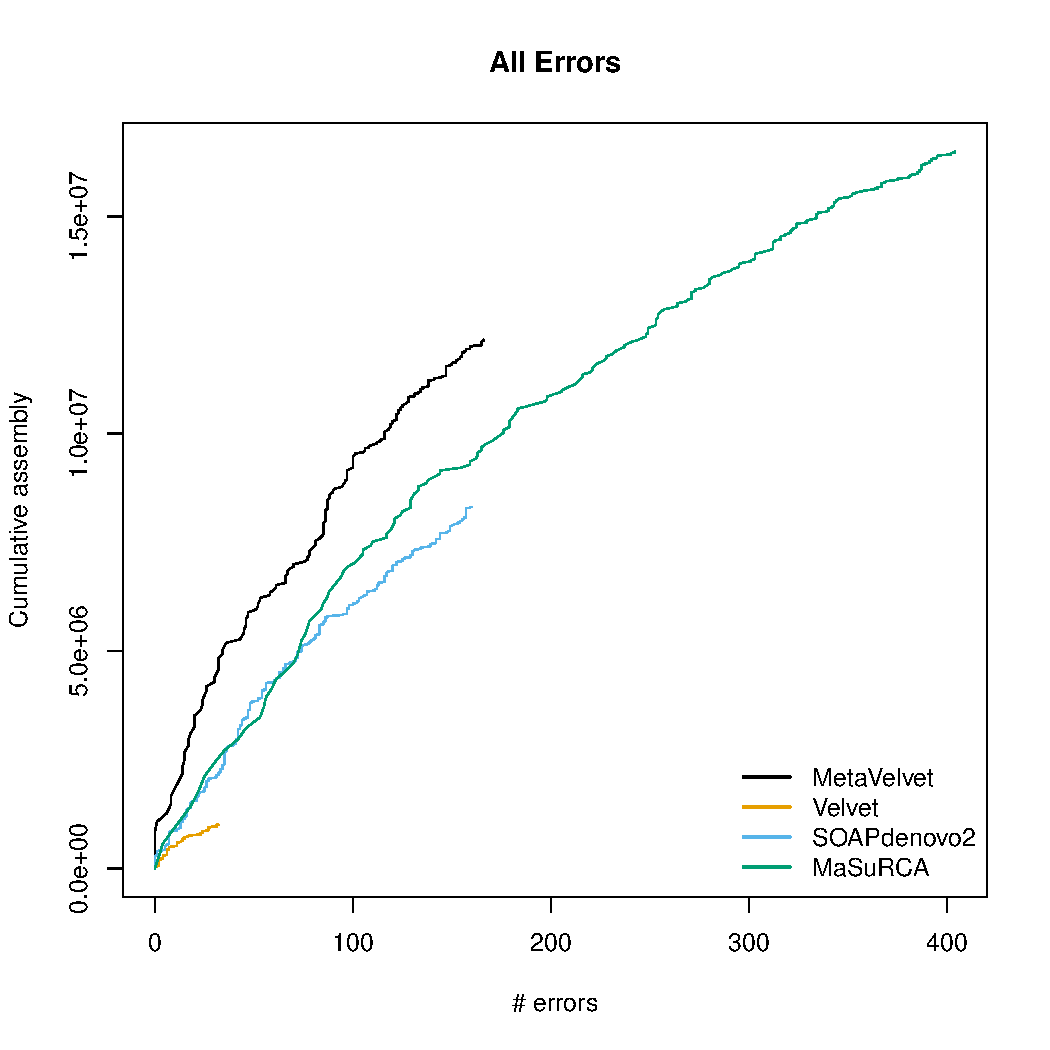
\includegraphics[width=3.86in]{figures/simulated_frc}
\end{center}
\caption[FRC plot of a simulated mock community]{FRC plot provided by VALET of a simulated mock community.}
\label{fig:mock_frc}
\end{figure}

\subsection{VALET accurately evaluates assemblies of a synthetic metagenomic community}

A major challenge of evaluating assemblies of environmental datasets is that a sizeable portion of the organsisms are unknown or lack a draft genome to compare against.
In silico simulations often lack the complexity and sequencing biases present in real environmental samples.
Fortunately, Shakya et al. provide a \emph{gold standard} synthetic metagenomic dataset containing a mixture of 64 organisms (16 members of Archaea and 48 organisms from 18 Bacteria phyla) with complete or high-quality draft genomes and 200-fold differences in abundances~\citep{shakya2013comparative}.
The dataset consists of 53.4 million reads (101 bp in length).
We assembled the dataset using Velvet~\citep{zerbino2008velvet}, MetaVelvet~\citep{namiki2012metavelvet}, SPAdes~\citep{bankevich2012spades}, and SOAPdenovo2~\citep{luo2012soapdenovo2} by MetAMOS~\citep{treangen2013metamos}.
We run VALET on the assemblies and compare the errors found with those reference-based mis-assemblies detected by QUAST (Table~\ref{synthetic_valet}).

%%%%%%%%%%%%%%%%%%%%%%%%%%%%%%
%% TODO Update assembly values
%%%%%%%%%%%%%%%%%%%%%%%%%%%%%%
While the MEGAHIT and Omega assemblies are close in total size (192.3 Mbp vs. 194 Mbp, respectively), MEGAHIT has nearly twice as many contigs as Omega (19,145 vs. 10,284).
QUAST detects far more mis-assemblies in the Omega assembly compared to MEGAHIT (56,917 vs. 770, respectively).
VALET detects 34.80\% and 96.10\% of these mis-assemblies found by QUAST in the MEGAHIT and Omega assemblies, respectively.
While Omega has a higher N50 than MEGAHIT (44.1 Kbp vs. 38.9 Kbp), after breaking at mis-assemblies, the N50 drops well below MEGAHIT's (11.9 Kbp vs. 33.5 Kbp), illustrating why the N50 metric is not always a good indicator of assembly quality.
VALET is able to accurately assess the quality of the two assemblies without using the reference genomes.

\subsection{Mis-assemblies not validated by QUAST}
%% Is this for the synthetic comminity?
We investigate the high false positive rate by examining a small number of regions flagged by VALET, but not marked by QUAST within the MEGAHIT assembly.
One contig, roughly 25 Kbp in size, had a 5 Kbp region at the start of the contig marked as high coverage (Figure~\ref{fig:rrna_coverages}).
This region was roughly 4x the median coverage of the remaining contig.
Using NCBI's BLAST~\citep{blast} and reference database, the region aligned to the organism \emph{Nostoc} sp. PCC 7120.
Upon closer inspection, this region contained 16S, 23S, and 5S rRNA genes and was found at \emph{four} locations in \emph{Nostoc} sp. PCC 7120.
This region was only found once in the assembly, so all the sequences from the repeats aligned to this region, inflating the coverage.
This noticeable and consistent increase in coverage caused VALET to mark it as mis-assembled.
Unsurprisingly, QUAST did not mark this as a mis-assembly because the actual sequence within this region matched the reference.

\begin{figure}[tb!]
\begin{center}
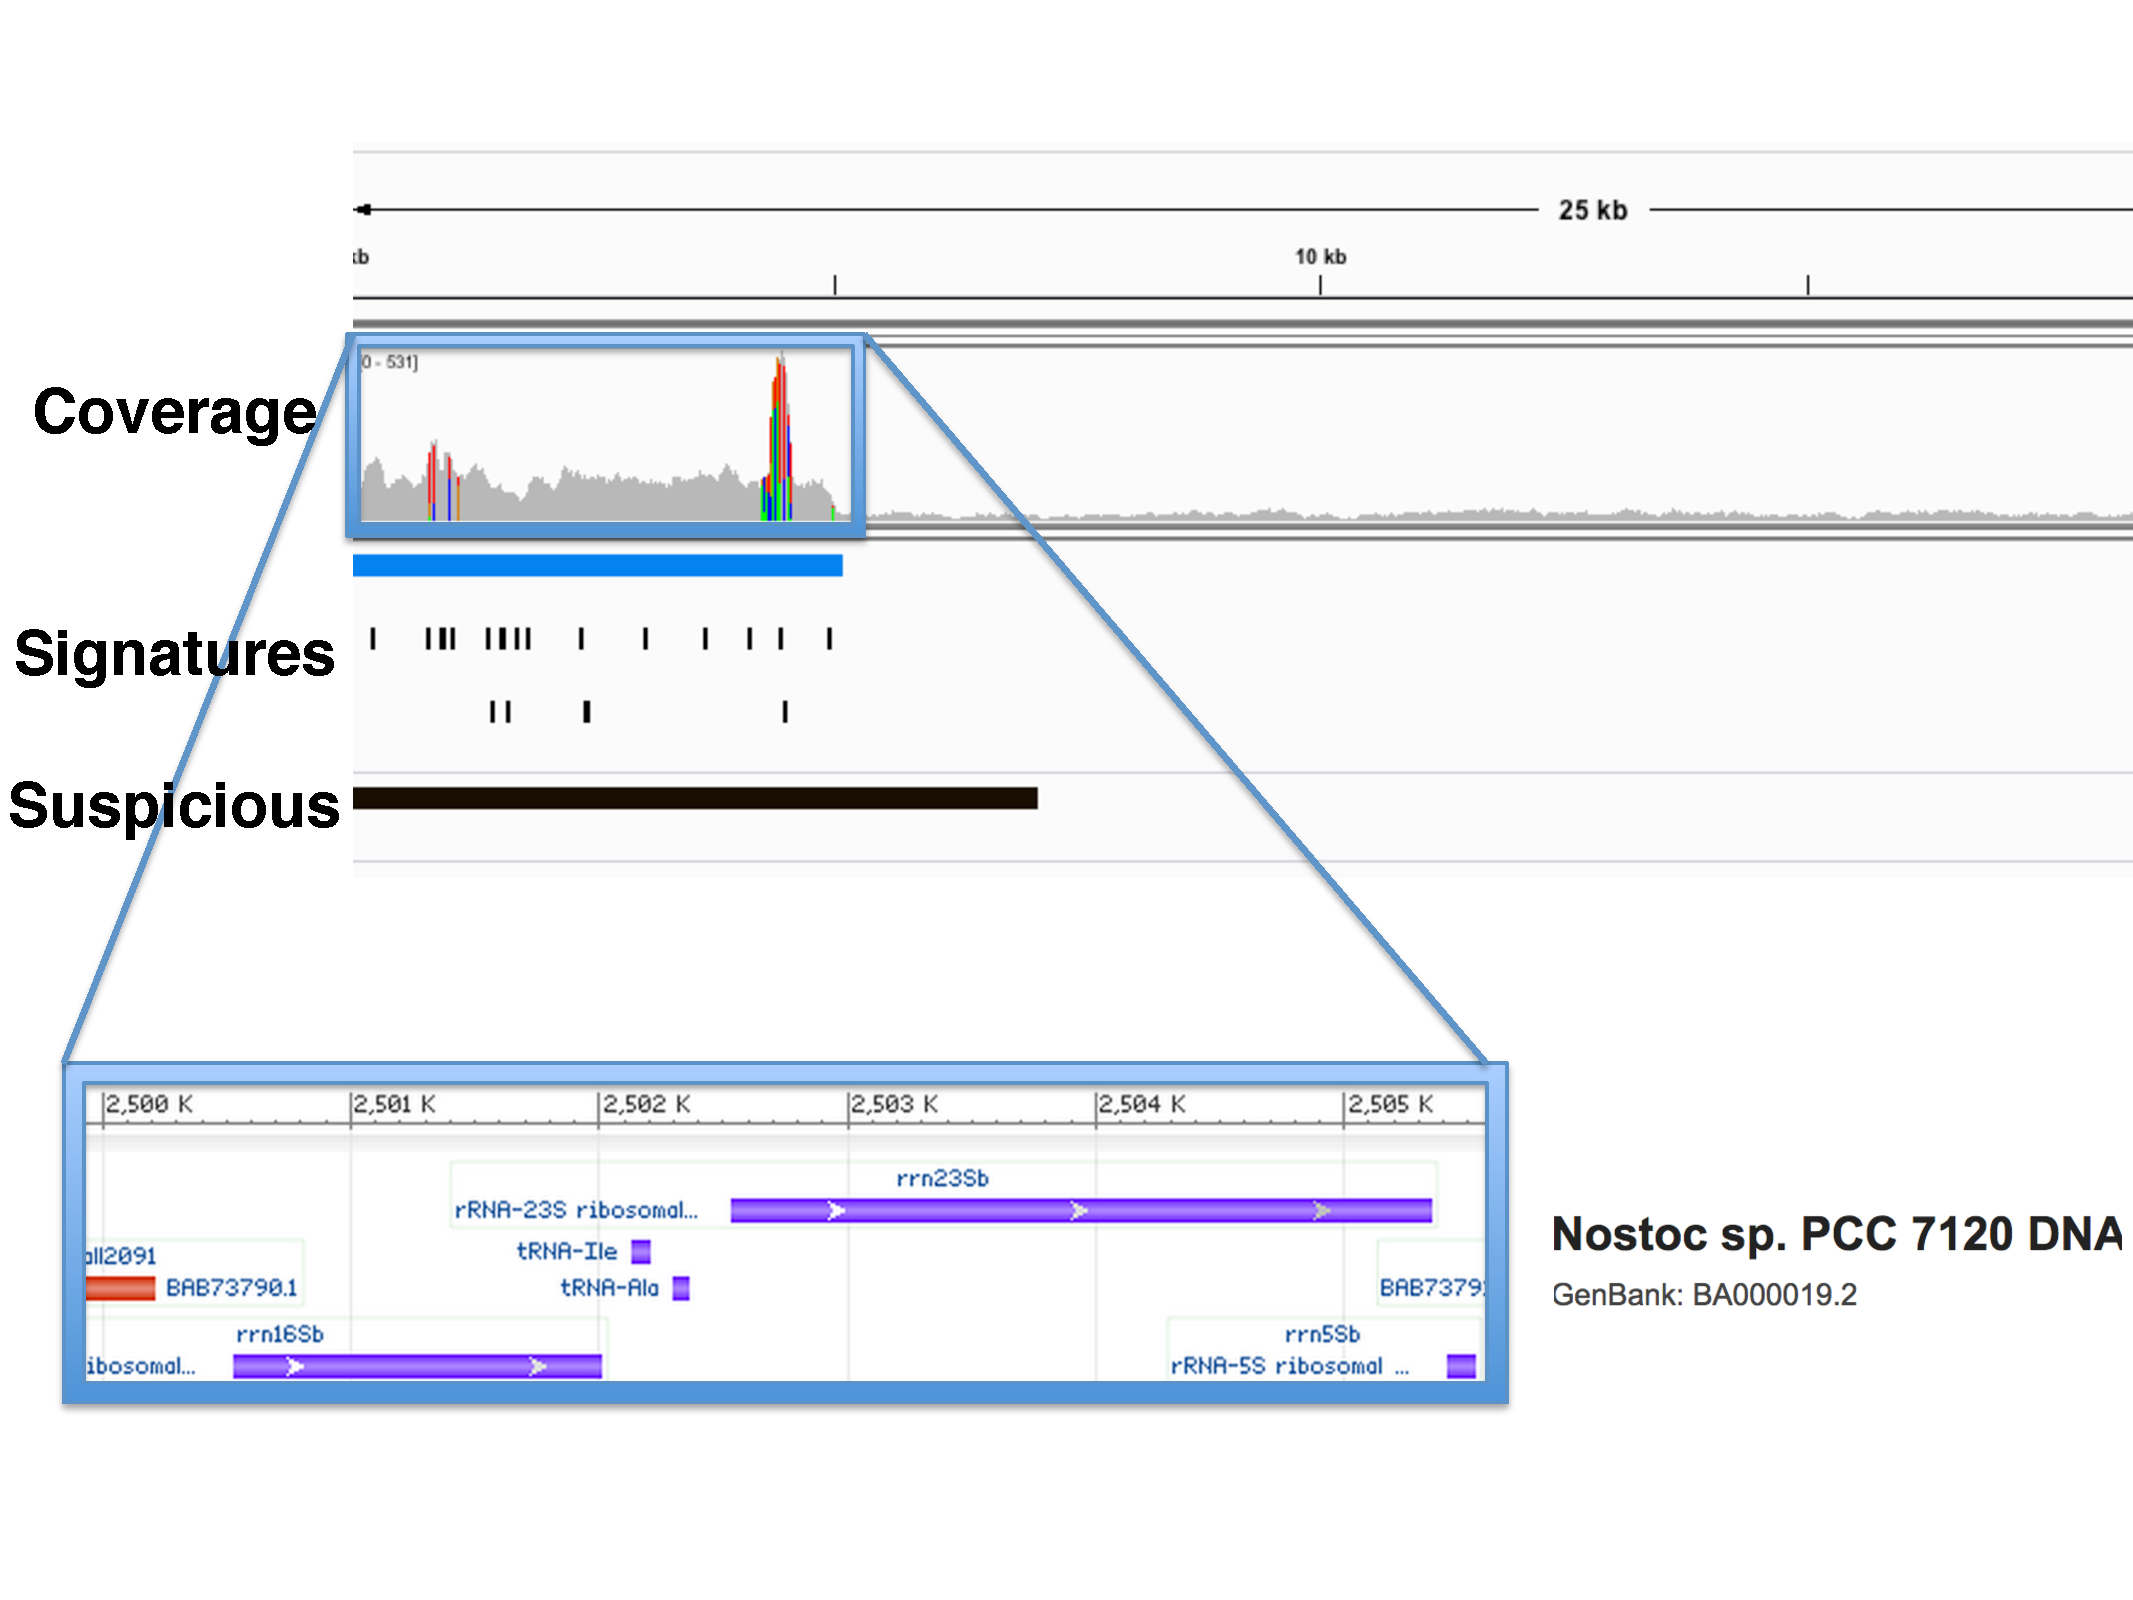
\includegraphics[width=\textwidth]{figures/rrna_coverages}
\end{center}
\caption[16S_rrna]{A closer examination of a region flagged by VALET, but no mis-assembly reported by QUAST. This region contained 16S, 23S, and 5S rRNA genes and was found at four locations in the \emph{Nostoc sp. PCC 7120 genome}.}
\label{fig:rrna_coverages}
\end{figure}

\section{Misassembly Example}
%%%%%
%%%% TODO add description to HMP sample
%%%%%
% \begin{figure*}[tb!]
% \begin{center}
% 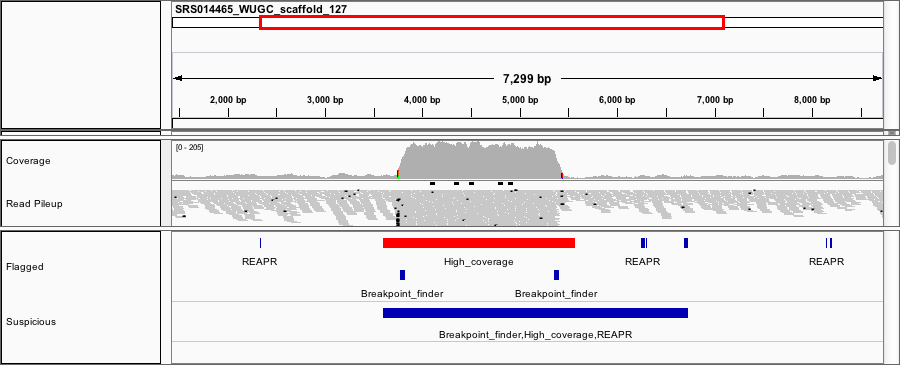
\includegraphics[width=.75\textwidth]{figures/hmp_plasmid}
% \end{center}
% \caption[hmp_plasmid]{An example suspicious region flagged by VALET in the HMP assembly of of a Vaginal introitus sample (SRS014465) from the Human Microbiome Project~\citep{human2012structure}.}
% \label{fig:hmp_plasmid}
% \end{figure*}

\bibliographystyle{natbib}
\bibliographystyle{achemnat}
\bibliographystyle{plainnat}
\bibliographystyle{abbrv}
\bibliographystyle{bioinformatics}

%\bibliographystyle{plain}

\bibliography{valet}

\end{document}
